\colorlet{species background color}{black!15}
\tikzset{
    x={1pt},
    y={-1pt},
    species background/.style={
        fill=species background color,
        draw=species background color,
        line width={1pt},
    },
    species label/.style={
        font=\bfseries,
        midway,
        anchor=west,
        align=left,
        xshift=10,
    },
    branch/.style={
        draw={#1},
        line width={0.5pt},
    },
    transfer branch/.style={
        branch={#1},
        -Stealth,
    },
    loss/.style={
        draw={#1}, cross out, thick,
        line width={0.5pt},
        inner sep=0pt,
        outer sep=0pt,
        minimum width={3},
        minimum height={3},
    },
    extant gene/.style 2 args={
        circle, fill={#1},
        outer sep=0pt, inner sep=0pt,
        minimum size={3},
        label={
            [font={\color{#1}},
                align=justify,
                inner xsep=4pt, inner ysep=0pt,
                outer xsep=0pt, outer ysep=0pt]
            right:#2
        },
    },
    extant gene/.default={black}{},
    branch node/.style={
        draw={#1}, fill={species background color!50!white},
        align=center,
        font={\color{#1}},
        outer sep=0pt, inner xsep=0pt, inner ysep=2pt,
        line width={0.5pt},
    },
    branch node/.default={black},
    speciation/.style={
        branch node={#1}, rectangle, rounded corners,
        inner xsep=4pt,
        minimum width={8},
        minimum height={8},
    },
    duplication/.style={
        branch node={#1}, rectangle,
        inner xsep=4pt,
        minimum width={8},
        minimum height={8},
    },
    horizontal gene transfer/.style={
        branch node={#1}, chamfered rectangle,
        chamfered rectangle sep={8 / 2.4},
        inner xsep=2pt,
        inner ysep=-1pt,
        minimum width={8},
        minimum height={8},
    },
}
\definecolor{reccolor0}{HTML}{000000}
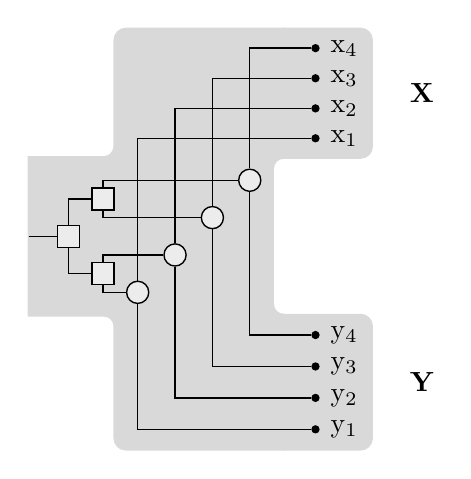
\begin{tikzpicture}
% background
\path[species background] (92.0,0) [rounded corners={4pt}] -- (31.0,0) -- (31.0,46.3799) [sharp corners] -- (0,46.3799) -- (0,103.3799) [rounded corners={4pt}] -- (31.0,103.3799) -- (31.0,151.8198) [sharp corners] -- (92.0,151.8198) -- (92.0,103.3799) [rounded corners={4pt}] -- (88.0,103.3799) -- (88.0,46.3799) [sharp corners] -- (92.0,46.3799) -- cycle;
\path[species background, rounded corners={4pt}] (92.0,0) -- (123.763,0) -- node[species label] {X} (123.763,46.3799) -- (92.0,46.3799);
\path[species background, rounded corners={4pt}] (92.0,103.3799) -- (123.763,103.3799) -- node[species label] {Y} (123.763,151.8198) -- (92.0,151.8198);
% gene branches
\path[branch={reccolor0}] (92.0,39.4749) -| (39.25,90.8799) (39.25,99.3799) |- (92.0,144.6398);
\path[branch={reccolor0}] (92.0,28.6649) -| (52.75,77.3799) (52.75,85.8799) |- (92.0,133.2798);
\path[branch={reccolor0}] (35.0,95.1299) -| (26.75,84.1299) (26.75,92.6299) |- (48.5,81.6299);
\path[branch={reccolor0}] (92.0,17.7849) -| (66.25,63.8799) (66.25,72.3799) |- (92.0,121.9198);
\path[branch={reccolor0}] (92.0,6.905) -| (79.75,50.3799) (79.75,58.8799) |- (92.0,110.5599);
\path[branch={reccolor0}] (62.0,68.1299) -| (26.75,57.1299) (26.75,65.6299) |- (75.5,54.6299);
\path[branch={reccolor0}] (10.0,74.8799) -- (0,74.8799);
\path[branch={reccolor0}] (22.5,88.3799) -| (14.25,70.6299) (14.25,79.1299) |- (22.5,61.3799);
\path[branch={reccolor0}] (102.0,39.4749) -- (92.0,39.4749);
\path[branch={reccolor0}] (102.0,28.6649) -- (92.0,28.6649);
\path[branch={reccolor0}] (102.0,17.7849) -- (92.0,17.7849);
\path[branch={reccolor0}] (102.0,6.905) -- (92.0,6.905);
\path[branch={reccolor0}] (102.0,144.6398) -- (92.0,144.6398);
\path[branch={reccolor0}] (102.0,133.2798) -- (92.0,133.2798);
\path[branch={reccolor0}] (102.0,121.9198) -- (92.0,121.9198);
\path[branch={reccolor0}] (102.0,110.5599) -- (92.0,110.5599);
% gene transfers
% events
\node[speciation={reccolor0}] at (39.25,95.1299) {};
\node[speciation={reccolor0}] at (52.75,81.6299) {};
\node[duplication={reccolor0}] at (26.75,88.3799) {};
\node[speciation={reccolor0}] at (66.25,68.1299) {};
\node[speciation={reccolor0}] at (79.75,54.6299) {};
\node[duplication={reccolor0}] at (26.75,61.3799) {};
\node[duplication={reccolor0}] at (14.25,74.8799) {};
\node[extant gene={reccolor0}{x\textsubscript{1}}] at (103.5,39.4749) {};
\node[extant gene={reccolor0}{x\textsubscript{2}}] at (103.5,28.6649) {};
\node[extant gene={reccolor0}{x\textsubscript{3}}] at (103.5,17.7849) {};
\node[extant gene={reccolor0}{x\textsubscript{4}}] at (103.5,6.905) {};
\node[extant gene={reccolor0}{y\textsubscript{1}}] at (103.5,144.6398) {};
\node[extant gene={reccolor0}{y\textsubscript{2}}] at (103.5,133.2798) {};
\node[extant gene={reccolor0}{y\textsubscript{3}}] at (103.5,121.9198) {};
\node[extant gene={reccolor0}{y\textsubscript{4}}] at (103.5,110.5599) {};
\end{tikzpicture}
